\subsection{Original statistical method and attempt history}\label{app:history-method}
The randomization seed is 20260923. The experimental unit is a trial, with pairing by block for treatment ratios. For each condition we report the arithmetic mean of its completed planned trials and a percentile bootstrap 95\% confidence interval using 10000 resamples of those trial indices. Conditions have ten completed trials except Redis-always publication, which has nine completions and one failed planned trial. That failure is reported separately, not assigned an artificial throughput or latency. A paired ratio is the ratio of resampled condition means under the same resampled block indices, not the mean of arbitrary per-message ratios. Comparisons involving a failed block use only the blocks completed by both conditions, so these are conditional-on-completion estimates. The bootstrap seed is fixed. These nominal, conditional confidence intervals summarize uncertainty in the condition mean under the working resampling assumption that completed block vectors are independent, identically distributed replicates. All blocks belong to one deployment campaign; their temporal dependence and the evolving storage history are not estimated away by resampling. They are not prediction intervals for individual runs, do not have proven exact finite-sample coverage here, and do not account for every systematic error or hardware population.

These are descriptive effect estimates, not a collection of significance tests with familywise error claims. We specify no $p$-value threshold, do not stop when an interval becomes favorable, and do not pool individual messages as independent replications. Recovery tables report all ten values through medians and ranges rather than presenting a high percentile from ten failure episodes as a precise tail estimate. No finite trial count can prove absence of all possible losses.

Additional post-observation diagnostics assess sensitivity without changing the primary dataset: leave-one-trial-out means for publication rates and within-trial p99 values; leave-one-common-block-out ratios for all thirteen paired effects; first-five versus last-five block summaries; and summaries between recorded execution interruptions. Leave-one-out ranges measure influence, not confidence coverage. Early/late contrasts and rank correlations with block order are descriptive, with no trend significance test or causal interpretation. The interruption segments follow planned trial ranges D001--D021, D022--D030, D031--D037, D038--D042, and D043--D060, using completed primary observations only. Their unequal, small cell counts prevent treating these segments as independent controlled replications. All computations and membership lists are retained.


\subsubsection{Protocol development and execution incidents}

The local protocol was written before main collection but was not externally preregistered. Twelve initial pilot trials were excluded. Before main collection, we added receive-request timestamps, increased the backlog from 4096 to 16384 messages after the pilot revealed short high-concurrency runs, and added the five-second primary durability series in place of relying on prefill timings. A final twelve-trial pilot verified the revised harness. Both pilot datasets and the prospective protocol versions are retained. The execution log records these changes; they are not presented as an immutable external registration.

During collection, a stream-creation request exceeded the five-second client deadline before a measured interval began. The server logged an 8.0186-second stream-creation handler. We retained that failed setup and the original logs, added checkpointed continuation, and retried the condition with unchanged settings and a fresh stream name. No completed measurement was replaced. After trial 88, a Redis-always warm-up returned through an error path and its cleanup also timed out, masking the primary operation error. Its original stack and log are retained. Administrative create, inventory, and deletion timeout settings were subsequently increased to 30~s. Redis default publication and acknowledgment socket timeouts and NATS response waits remained 5~s; the blocking-read overrides documented in Section~\ref{sec:client-waits} were unchanged. The durability series also stopped after 21 completed trials when a NATS-always warm-up publication timed out; the server logged approximately 4.9925~s in deletion/read-loop processing for that warm-up stream. No timed sample for its next condition had begun. We preserved the original log and all completed samples, then added append-only continuation to that series without changing its measurement path or deadlines. A further NATS-always warm-up publication timed out after 30 completed durability trials, with a corresponding 3.5595~s deletion/read-loop warning; the existing checkpointed binary then continued without a further code change. The causes of these interruptions are not established. Setup and warm-up availability are therefore reported separately from timed outcomes.

Planned timed-publication trial D038 (Redis-always) subsequently aborted with a socket read timeout. Its partial client timings and confirmed-request count were lost on process abort and cannot be reconstructed from the retained evidence. A later retained-state snapshot contained 1568 distinct application IDs and zero pending consumer acknowledgments; this cannot identify which publications the client had confirmed. We preserve the failure as the planned outcome and exclude its unavailable throughput and latency from completed-run estimates. An orchestration error during failure-ledger copying caused an unintended completed replay of D038; that replay is retained but excluded from primary statistics. Stopping that continuation also caused an operator interruption of D043, whose partial broker state was preserved and whose planned condition was rerun after cleanup. These operational deviations and the exact evidence are recorded in the artifact. No observed slow completed planned trial was removed. A plot of publication throughput by block was added as a descriptive diagnostic after observing this variability; it is not a preregistered hypothesis test.

Table~\ref{tab:attempt-outcomes} consolidates the 550 planned outcomes and six additional documented attempts. Its accompanying record-level inventory links each entry to retained evidence and leaves unavailable times and confirmation counts missing. Successful warm-ups are part of their completed attempts, not additional rows. The two excluded twelve-trial pilots and infrastructure provisioning are outside this inventory. This is retrospective accounting of known execution outcomes, not a prospective exclusion rule or a denominator for estimating setup availability or total workload-completion cost. In particular, the later successful D043 attempt cannot reconstruct the interrupted attempt's client history.

\begin{table}[htbp]
\centering\small
\begin{tabular}{L{.40\linewidth}rL{.43\linewidth}}
\toprule
Retained outcome & Count & Treatment in this study\\
\midrule
Completed timing trials & 419 & 300 drain, 59 publication, 60 serial\\
Active consumer recovery & 120 & Recovered identifiers and cleared pending state\\
No-reclaimer controls & 10 & Pending at reconciliation; nominal budgets only\\
Planned publication failure & 1 & D038; client timings unavailable\\
\midrule
Additional setup failure & 1 & Tmain052; excluded from timed estimates\\
Additional warm-up failures & 3 & Tmain089, D022, D031; timed trials not begun\\
Operator interruption & 1 & D043; interrupted client trace unavailable\\
Completed diagnostic replay & 1 & D038; retained and excluded from estimates\\
\bottomrule
\end{tabular}

\caption{Retained campaign outcomes and additional documented attempts. The first four rows account for all 550 planned outcomes. The remaining six attempts are separate from those outcomes. Counts do not reconstruct missing durations or establish end-to-end availability.}
\label{tab:attempt-outcomes}
\end{table}
\FloatBarrier


\subsection{Original campaign results}\label{app:history-results}
\subsubsection{Recorded outcomes and evidence quality}
All 300 planned backlog-drain trials completed and their \MainMessages{} message records passed complete identifier-set, uniqueness, retained-count, and pending-state checks. The 60 serial sensitivity trials similarly reconciled \SerialMessages{} messages. The primary publication series has 59 completed planned trials with \TimedMessages{} confirmed appends and one retained Redis-always timeout. Its accidental completed replay is excluded as specified in Section~\ref{sec:method}. Publication-only integrity checks establish the retained count, not a complete payload readback. The analyzer reconstructs each reported throughput and percentile from raw timings and rejects inconsistent summaries or a missing failure ledger.

All 120 active recovery episodes returned the original identifier, acknowledged it, and left one retained message with zero pending acknowledgments; JetStream reported two deliveries in each episode. All ten Redis no-reclaimer controls remained pending at the end of their observation windows. Every victim exit was recorded as killed by a signal. The largest kill-invocation-to-observed-exit bracket was \KillBracket{}\,ms. The final seven-pod snapshot reported zero container restarts and zero cgroup OOM kills. Recorded driver CPU-counter differences showed no throttling within completed timed trials; this does not establish an idle testbed or identify the cause of the recorded timeouts.

\subsubsection{RQ1: failure age, reclamation, and observed redelivery}

\begin{table}[htbp]
\centering\small
\begin{tabular}{rrlrrr}
\toprule
$\Delta$ & $\alpha$ & System / sleep & $\Delta(1-\alpha)$ & Median & Range\\
 & & & (ms) & (ms) & (ms)\\
\midrule
250 & 0.1 & JetStream & 225.0 & 226.5 & [225.9, 226.9]\\
250 & 0.1 & Redis / 10 ms & 225.0 & 230.2 & [228.4, 234.3]\\
250 & 0.1 & Redis / 100 ms & 225.0 & 265.4 & [234.0, 313.9]\\
250 & 0.75 & JetStream & 62.5 & 63.6 & [63.1, 64.5]\\
250 & 0.75 & Redis / 10 ms & 62.5 & 67.9 & [63.9, 70.6]\\
250 & 0.75 & Redis / 100 ms & 62.5 & 134.0 & [75.8, 161.2]\\
1000 & 0.1 & JetStream & 900.0 & 907.1 & [905.4, 910.2]\\
1000 & 0.1 & Redis / 10 ms & 900.0 & 903.5 & [900.4, 913.7]\\
1000 & 0.1 & Redis / 100 ms & 900.0 & 943.5 & [911.7, 981.1]\\
1000 & 0.75 & JetStream & 250.0 & 257.9 & [255.5, 260.6]\\
1000 & 0.75 & Redis / 10 ms & 250.0 & 255.4 & [251.2, 269.4]\\
1000 & 0.75 & Redis / 100 ms & 250.0 & 319.4 & [258.9, 339.4]\\
\bottomrule
\end{tabular}

\caption{Failure-to-redelivery latency for all recovery configurations. Each row contains ten killed-consumer episodes. $\Delta(1-\alpha)$ is a nominal reference based on the scheduled age after client receipt, not a verified server-side lower bound. Ranges contain the minimum and maximum observed episode.}
\label{tab:recovery}
\end{table}

\begin{figure}[htbp]
\centering
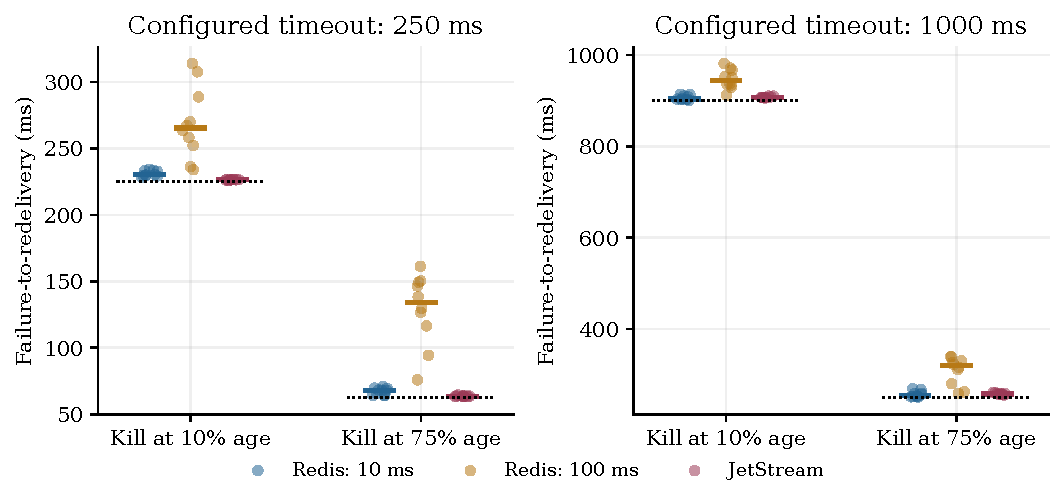
\includegraphics[width=\linewidth]{figures/recovery.pdf}
\caption{Every active-reclamation recovery observation. Horizontal colored marks show medians; horizontal jitter separates points and has no numerical meaning. Dotted lines show the nominal client-receipt-based residual-time reference. The ten no-reclaimer controls are censored and are reported separately rather than plotted as exact recovery times.}
\label{fig:recovery}
\end{figure}
Table~\ref{tab:recovery} and Figure~\ref{fig:recovery} report shorter failure-to-redelivery intervals after later kills at the same configured timeout. At $\Delta=250$\,ms, the nominal remaining intervals are 225 and 62.5\,ms. JetStream's corresponding medians are 226.5 and 63.6\,ms; Redis with a 10\,ms reclaim sleep yields 230.2 and 67.9\,ms. At $\Delta=1000$\,ms, the medians decrease from 907.1 to 257.9\,ms for JetStream and from 903.5 to 255.4\,ms for Redis with the shorter sleep. This direction is consistent with the residual-time decomposition in Theorem~\ref{thm:recovery}: later failure leaves less of the existing eligibility interval to wait out. Eligibility depends on message age and acknowledgment state; it can arise while a consumer remains alive. These observations do not establish a death-detection mechanism or directly observe the broker-side timer origin.

Redis reclamation frequency also matters. With a 100\,ms sleep, the late-failure median rises to 134.0\,ms at the 250\,ms timeout and 319.4\,ms at the 1000\,ms timeout. Across the four age/timeout cells, the median observed excess $(\widehat r-\widehat d)-\Delta$ ranges from 4.0 to 6.2\,ms with a 10\,ms sleep, compared with 40.7--72.2\,ms with a 100\,ms sleep. JetStream's median excess ranges from 1.9 to 8.6\,ms. Neither a configured sleep nor an observed maximum is a proven future scheduling bound. JetStream's 1000\,ms medians are slightly above the shorter-sleep Redis medians, so the results do not support an unconditional claim that one system recovers faster.

The negative controls isolate a separate mechanism: ten observed non-recoveries with pending state intact are consistent with Proposition~\ref{prop:no-reclaim}. Their finite observation procedures do not empirically prove infinite non-delivery; the proposition supplies that conditional counterexample from the stated new-read-only policy. Because exact censor endpoints were not recorded, these controls contribute descriptive evidence rather than exposure-time or survival estimates. The answer to RQ1 is therefore twofold: a failure leaves a residual timeout, and actual recovery additionally depends on reclamation or expiry selection and available demand. Under the active policies studied, all episodes recovered; without Redis reclamation, none of the controls did during observation.

\subsubsection{RQ2: concurrency gains and cycle-latency cost}

\begin{table}[htbp]
\centering\small\setlength{\tabcolsep}{4pt}
\begin{tabular}{llrrr}
\toprule
System & Mode & $X_1$ (kmsg/s) & $X_{16}$ (kmsg/s) & $X_{16}/X_1$\\
\midrule
Redis & memory & 2.89 [2.74, 3.01] & 36.37 [35.94, 36.83] & 12.59 [12.13, 13.15]\\
Redis & periodic & 2.66 [2.56, 2.76] & 29.32 [27.73, 30.50] & 11.02 [10.22, 11.79]\\
Redis & always & 0.29 [0.29, 0.30] & 2.51 [2.47, 2.55] & 8.59 [8.47, 8.72]\\
JetStream & memory & 2.30 [2.26, 2.34] & 29.79 [29.43, 30.12] & 12.94 [12.69, 13.23]\\
JetStream & periodic & 2.27 [2.24, 2.29] & 28.03 [26.89, 28.97] & 12.36 [11.79, 12.83]\\
JetStream & always & 2.24 [2.21, 2.27] & 27.43 [27.04, 27.83] & 12.24 [11.98, 12.54]\\
\bottomrule
\end{tabular}

\caption{Acknowledged backlog-drain throughput at one and sixteen consumers, with means and nominal 95\% bootstrap intervals. Speedup is the ratio of condition means with a paired block-bootstrap interval. Each condition contains ten trials.}
\label{tab:concurrency}
\end{table}

\begin{figure}[htbp]
\centering
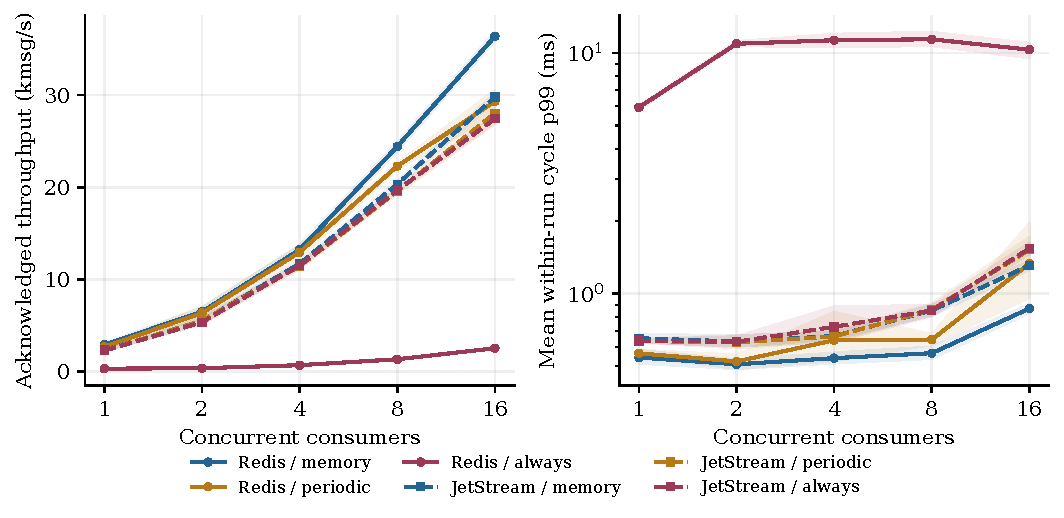
\includegraphics[width=\linewidth]{figures/concurrency.pdf}
\caption{The complete concurrency response. Lines connect measured consumer counts without estimating unmeasured counts. Shaded bands are nominal 95\% bootstrap confidence intervals for condition means; the right panel uses a logarithmic latency axis. Cycle latency is successful receive-request invocation to acknowledgment completion.}
\label{fig:concurrency}
\end{figure}
Increasing $C$ from one to sixteen improved mean drain throughput in every profile (Table~\ref{tab:concurrency}). Redis gains were \RedisMemorySpeedup{}, \RedisPeriodicSpeedup{}, and \RedisAlwaysSpeedup{} times for memory, periodic, and always modes; JetStream gains were \NatsMemorySpeedup{}, \NatsPeriodicSpeedup{}, and \NatsAlwaysSpeedup{} times. All six endpoint gains are below the sixteenfold increase in workers. The memory profiles reached 36.37\,kmsg/s for Redis and 29.79\,kmsg/s for JetStream at sixteen consumers. Periodic profiles reached 29.32 and 28.03\,kmsg/s. These rates describe the measured request/acknowledgment path with a prefilled backlog, not a server-capacity ceiling or an open-loop saturation point.

The throughput gain has a cycle-latency cost. From one to sixteen consumers, mean within-trial cycle p99 increased from 0.543 to 0.867\,ms for Redis memory and from 0.653 to 1.310\,ms for JetStream memory. Redis periodic increased from 0.565 to 1.334\,ms and JetStream periodic from 0.636 to 1.520\,ms. Redis always increased from 5.942 to 10.311\,ms, while JetStream always increased from 0.636 to 1.541\,ms. In contrast, the corresponding common-start-to-receipt drain p99 values decrease between these endpoints (the complete matrix below): more workers complete the backlog sooner despite a slower individual cycle.

Reconstructed occupancy $U$ lies between 0.9936 and 0.9995 across all 300 trials. Every worker's recorded intervals are nonoverlapping and inside the measured window, satisfying the checked premises of Theorem~\ref{thm:concurrency}. Thus recorded successful cycles occupy nearly all available worker time. The identity $X=CU/\overline R$ explains how increased mean cycle cost offsets the added concurrency; it does not identify which internal contention mechanism caused that cost. Nor does a p99 value replace $\overline R$ in this identity.

The always-mode endpoint is particularly easy to misread: JetStream drains 27.43\,kmsg/s and Redis 2.51\,kmsg/s, but their consumer-state synchronization contracts differ. RQ2 is answered by sublinear endpoint scaling with rising cycle tails within each profile. A cross-system ranking under an equal synchronous consumer-progress durability guarantee is not established by these configurations.

\subsubsection{RQ3: confirmed-publication cost under persistence policies}

\begin{table}[htbp]
\centering\small\setlength{\tabcolsep}{4pt}
\begin{tabular}{llrrrr}
\toprule
System & Mode & $n$ & Throughput (kmsg/s) & p50 (ms) & p99 (ms)\\
\midrule
Redis & memory & 10 & 73.90 [73.60, 74.19] & 0.204 & 0.474 [0.466, 0.486]\\
Redis & periodic & 10 & 61.38 [61.08, 61.67] & 0.247 & 0.557 [0.551, 0.565]\\
Redis & always & 9 & 3.03 [1.73, 4.31] & 9.959 & 29.001 [11.615, 50.929]\\
JetStream & memory & 10 & 60.38 [58.99, 61.32] & 0.241 & 0.704 [0.678, 0.742]\\
JetStream & periodic & 10 & 49.49 [48.29, 50.48] & 0.281 & 0.849 [0.832, 0.869]\\
JetStream & always & 10 & 0.37 [0.19, 0.56] & 108.664 & 579.568 [91.362, 1,459.647]\\
\bottomrule
\end{tabular}

\caption{Five-second publication workload with sixteen independent publishers. Throughput and p99 entries give means and nominal 95\% bootstrap intervals; p50 entries are means of within-trial medians. $n$ is the number of completed planned trials out of ten; the failed Redis-always trial is reported separately.}
\label{tab:durability}
\end{table}

\begin{figure}[htbp]
\centering
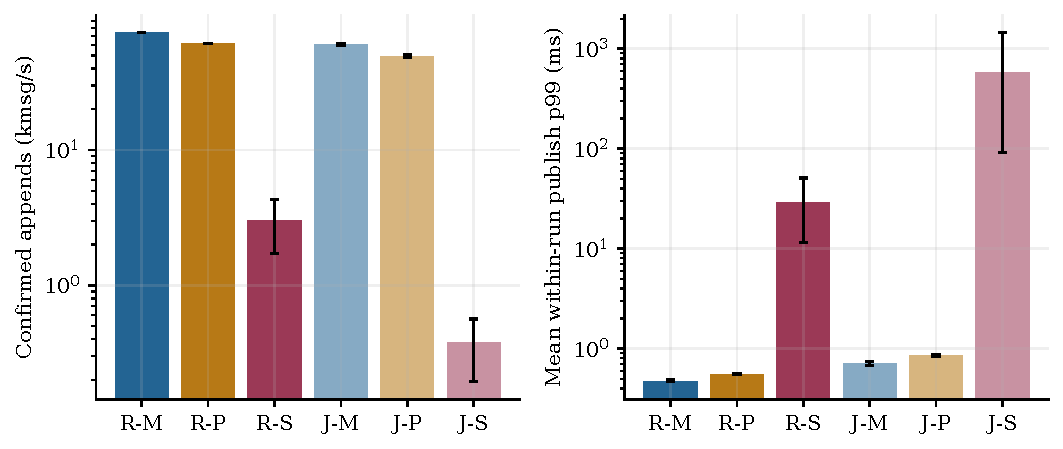
\includegraphics[width=\linewidth]{figures/durability.pdf}
\caption{Confirmed-publication throughput and latency for Redis (R) and JetStream (J), in memory (M), periodic (P), and always (S) profiles. Both vertical axes are logarithmic. Error bars give nominal 95\% bootstrap confidence intervals for means conditional on completion (nine Redis-always trials and ten for each other profile).}
\label{fig:durability}
\end{figure}
The periodic configurations exhibited lower confirmed-publication throughput than the memory configurations in this campaign. Memory and periodic means were 73.90 and 61.38\,kmsg/s for Redis, and 60.38 and 49.49\,kmsg/s for JetStream. The paired periodic/memory throughput ratios were 0.8305 [0.8237, 0.8371] for Redis and 0.8197 [0.7933, 0.8511] for JetStream, using nominal 95\% block-bootstrap intervals. Mean within-trial publication p99 was 0.474 versus 0.557\,ms and 0.704 versus 0.849\,ms, respectively. These descriptive differences include the evolving storage history and shared environment; they do not isolate the causal cost of synchronization policy or measure power-loss data loss.

Always-mode publication was substantially slower and more variable. The nine completed planned Redis-always trials averaged 3028\,msg/s [1725, 4306], with a mean within-trial p99 of 29.0\,ms [11.6, 50.9]. The tenth planned trial timed out at the measured request deadline and has no reconstructible client latency sample. The ten completed JetStream-always trials averaged 375\,msg/s [194, 564], with a mean within-trial p99 of 579.6\,ms [91.4, 1459.6]. The wide intervals and per-block observations in Figure~\ref{fig:durability-blocks} are material results: the point estimates should not be presented as stable production tail-latency guarantees. The separately recorded setup and warm-up incidents further constrain operational interpretation.

\begin{table}[htbp]
\centering\small\setlength{\tabcolsep}{3.5pt}
\begin{tabular}{llrrrr}
\toprule
System & Mode & Mean p99 & Median p99 & LOO means & Early / late rate\\
 & & (ms) & (ms) & (ms) & (kmsg/s)\\
\midrule
Redis & memory & 0.47 & 0.47 & [0.47, 0.48] & 73.98 / 73.83\\
Redis & periodic & 0.56 & 0.56 & [0.56, 0.56] & 61.38 / 61.37\\
Redis & always & 29.00 & 7.46 & [20.15, 32.10] & 3.78 / 2.08\\
JetStream & memory & 0.70 & 0.68 & [0.69, 0.71] & 59.68 / 61.07\\
JetStream & periodic & 0.85 & 0.84 & [0.84, 0.85] & 50.35 / 48.64\\
JetStream & always & 579.57 & 160.26 & [150.53, 639.37] & 0.45 / 0.30\\
\bottomrule
\end{tabular}

\caption{Post-observation publication sensitivity. The mean and median summarize completed trials' p99 values. LOO gives the range of means after omitting each completed trial in turn, solely as an influence diagnostic. Early and late rates use blocks 1--5 and 6--10. Redis-always has five early and four late completions; other cells have five in each half. No observation is removed from primary estimates.}
\label{tab:robustness}
\end{table}

Table~\ref{tab:robustness} shows the sensitivity of always-mode summaries. JetStream-always's mean within-trial p99 is \NatsAlwaysPnnMean{}\,ms, whereas the median of those ten p99 values is \NatsAlwaysPnnMedian{}\,ms. Its leave-one-out means range from \NatsAlwaysPnnLooMin{} to \NatsAlwaysPnnLooMax{}\,ms; the minimum omits D040, whose within-trial p99 is 4440.9\,ms. Redis-always's corresponding mean and median are \RedisAlwaysPnnMean{} and \RedisAlwaysPnnMedian{}\,ms. These contrasts characterize influence and skew, not grounds for discarding slow observations.

\begin{table}[htbp]
\centering\small\setlength{\tabcolsep}{4pt}
\begin{tabular}{llrrr}
\toprule
System & Mode & Trials & Messages per trial & Positions above p99\\
\midrule
Redis & memory & 10 & 365,505--372,128 & 3,655--3,721\\
Redis & periodic & 10 & 303,669--310,204 & 3,036--3,102\\
Redis & always & 9 & 2,608--26,221 & 26--262\\
JetStream & memory & 10 & 273,779--310,872 & 2,737--3,108\\
JetStream & periodic & 10 & 243,055--257,750 & 2,430--2,577\\
JetStream & always & 10 & 149--3,577 & 1--35\\
\bottomrule
\end{tabular}

\caption{Sample information underlying completed publication trials' empirical p99 values. Ranges span the retained trials of each profile. Positions above p99 are $N-\lceil0.99N\rceil$ and do not imply independent tail observations.}
\label{tab:tail-counts}
\end{table}

Table~\ref{tab:tail-counts} makes the unequal sample sizes explicit. All 59 trial counts, ranks, and p99 values are retained in \artifact{data/derived/publication-tail-samples.csv}. D040 contains 149 confirmed publications, so its p99 is order statistic 148, the second-largest observation. Its influential tail estimate consequently has very little information above the selected rank. The mean of trial p99 values remains a descriptive summary of these observed trials; it is weak evidence for a stable population tail, and equal trial weights do not equalize percentile precision. Longer, independently repeated observations would be required for a stronger tail characterization. We retain D040 and do not replace its percentile with a pooled-message estimate.

The direction of all thirteen reported paired contrasts survives every leave-one-common-block-out calculation. Magnitudes remain conditional on the retained blocks: the periodic/memory publication ratios range from 0.8285 to 0.8320 for Redis and from 0.8076 to 0.8282 for JetStream in that diagnostic. Early versus late always-mode throughput declines from 3.78 to 2.08\,kmsg/s for Redis and from 0.45 to 0.30\,kmsg/s for JetStream. A simple monotonic degradation model is also insufficient: JetStream-always averages 483.3\,msg/s in D001--D021, 24.6\,msg/s in the interruption-bounded D038--D042 segment containing its single D040 observation, and 462.7\,msg/s in D043--D060. The artifact reports every segment and cell count. These uncontrolled contrasts establish variability and sensitivity to execution history, not that an interruption or AOF growth caused a particular outcome. Independent campaign repetitions are needed to assess repeatability beyond this deployment.


Against memory mode, the paired always/memory throughput ratio is 0.0410 [0.0233, 0.0583] for Redis over nine common completed blocks and 0.00621 [0.00318, 0.00945] for JetStream over ten blocks. Their reciprocal point estimates are \RedisSyncSlowdown{}- and \NatsSyncSlowdown{}-fold slowdowns. Because the Redis estimate excludes an unavailable failed-trial metric, it describes successful runs and can understate the operational cost of the complete outcome distribution. We neither impute zero throughput nor replace the failed outcome with its diagnostic replay.

The original serial-publisher sensitivity gives a different view (Appendix~\ref{app:serial}): always-mode publication averaged 603\,msg/s [591, 614] for Redis and 585\,msg/s [565, 598] for JetStream. The close point estimates do not establish equivalence. This shorter fixed-count workload differs in both publication concurrency and duration, so it cannot isolate batching as the cause of the contrast with the sixteen-publisher results. No syscall or storage-device trace was collected in that original campaign to establish the mechanism. The follow-up's matched-duration publication and syscall diagnostics are a separate dataset.

RQ3 is therefore answered as a descriptive, workload-specific tradeoff: the configured periodic profiles preserve most memory-mode throughput with modestly higher observed tails, whereas always-mode confirmed publication incurs much larger and more variable observed costs in this shared Btrfs/NVMe environment. The synchronization contract, accumulated storage history, completion conditioning, and failure class must accompany that performance statement. Neither these append measurements nor the fast JetStream drain acknowledgments prove equivalent durable consumer progress or stable-media survival after a power cut.

\begin{figure}[htbp]
\centering
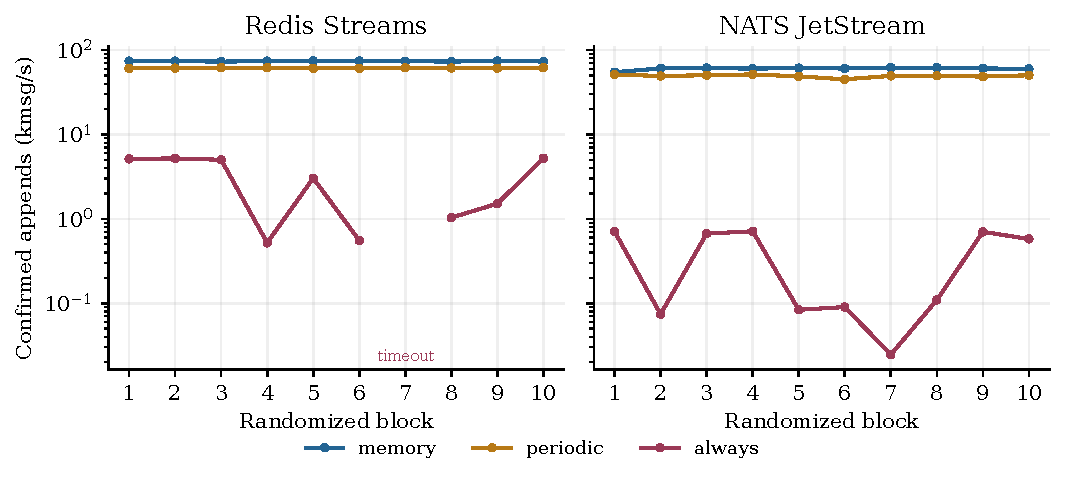
\includegraphics[width=\linewidth]{figures/durability-blocks.pdf}
\caption{Descriptive publication-throughput diagnostic by randomized block. Each point is one completed planned trial. The timeout annotation has no throughput coordinate and identifies the failed Redis-always trial in block seven. A missing value interrupts its line; no failure is imputed as zero. Blocks are ordered experimental groups, not equal wall-time intervals.}
\label{fig:durability-blocks}
\end{figure}
